\begin{frame}
    \frametitle{参数自适应}

    考虑一个简单的自适应控制系统:

    \[
    \begin{cases}
    \dot{e} = -e + \theta w(t) \\
    \dot{\theta} = -e w(t)
    \end{cases}
    \]

    其中,\( e \) 是跟踪误差,\( \theta \) 是参数误差,\( w(t) \) 是一个有界连续函数。
\end{frame}

\begin{frame}
考虑下方有界函数:
\[
\begin{split}
V &= e^2 + \theta^2 \\
\dot{V} &= 2e(-e + \theta w) + 2\theta(-ew(t)) = -2e^2 \leq 0
\end{split}
\]
所以 \( V(t) \geq V(0) \),因此 \( e \) 和 \( \theta \) 是有界的。

由于动力学是非自治的,不变集定理不能用来推断 \( e \) 的收敛性。

为了使用 Barbalat 引理,检查 \( \dot{V} \) 的一致连续性。
\[
\ddot{V} = -4e(-e + \theta w)
\]

\( \ddot{V} \) 是有界的,因为根据假设 \( w \) 是有界的,且 \( e \) 和 \( \theta \) 已被证明是有界的 \( \rightsquigarrow \dot{V} \) 是一致连续的。

应用 Barbalat 引理:当 \( \dot{V} = 0 \) 时,\( t \to \infty \) 时 \( e \to 0 \)。

\textbf{重要提示}:尽管 \( e \to 0 \),但系统不是渐近稳定(a.s.)的,因为仅证明了 \( \theta \) 是有界的。
\end{frame}


\begin{frame}
    \frametitle{闭环系统是否稳定}

    \begin{enumerate}
        \item 持续激励信号:$w(t)=\sin(t)$
        \item 非持续激励信号:当 $t< 5$ 时,$w(t)=1$;当$t\geq 5$时,$w(t)=0$
    \end{enumerate}

    \begin{figure}
        \begin{subfigure}[b]{0.45\textwidth}
            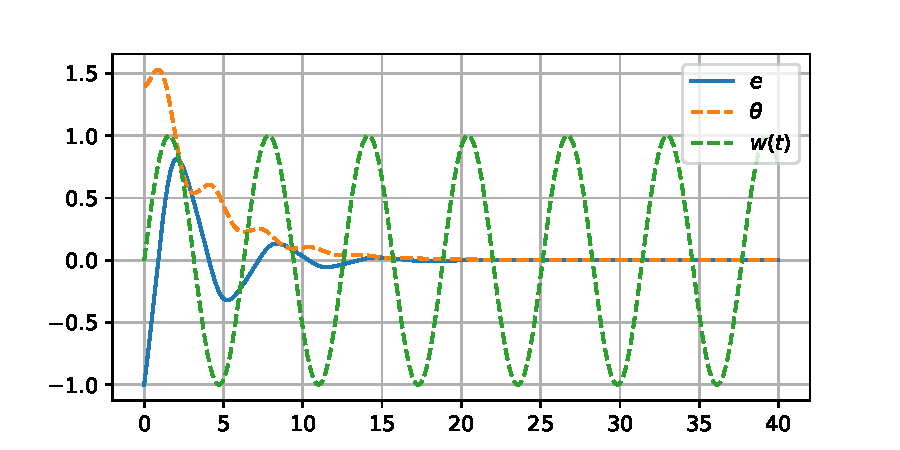
\includegraphics[width=\linewidth]{figure/simple-pe.pdf}
            \caption{持续激励信号下}
        \end{subfigure}
        \begin{subfigure}[b]{0.45\textwidth}
            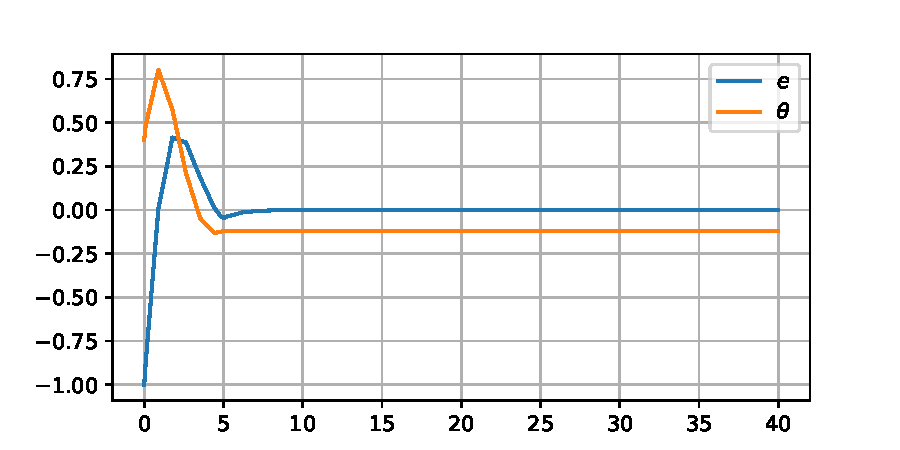
\includegraphics[width=\linewidth]{figure/simple-npe.pdf}
            \caption{非持续激励信号}
        \end{subfigure}
    \end{figure}
\end{frame}